General equation of second degree is given by :
\begin{align}
\vec{x}^T\vec{V}\vec{x}+2\vec{u}^T\vec{x}+f=0\label{eq:solutions/41/18/eq:1}
\end{align}
In the vector form \eqref{eq:solutions/41/18/eq:0} can be written as :
\begin{align}
\vec{x}^T\myvec{1&\frac{1}{2}\\[0.1cm]\frac{1}{2}&1}\vec{x}+2\myvec{\frac{1}{2}\\[0.1 cm]\frac{1}{2}}^T\vec{x}-1=0\label{eq:solutions/41/18/eq:2}
\end{align}
By comparing \eqref{eq:solutions/41/18/eq:1} and \eqref{eq:solutions/41/18/eq:2} we get : 
\begin{align}
    \vec{V}=\myvec{1&\frac{1}{2}\\[0.1cm]\frac{1}{2}&1},\vec{u}=\myvec{\frac{1}{2}\\[0.1 cm]\frac{1}{2}},f=-1\label{eq:solutions/41/18/eq:3}
\end{align}
Eigen values for matrix $\vec{V}$ can be calculated by solving :  
\begin{align}
    \mydet{1-\lambda&\frac{1}{2}\\[0.1cm]\frac{1}{2}&1-\lambda}&=0\\
    \lambda^2-2\lambda+\frac{3}{4}&=0\\
    \lambda_1=\frac{3}{2},\lambda_2&=\frac{1}{2}
\end{align}
By doing Eigenvalue Decomposition and Affine Transformation we get : 
\begin{align}
    \vec{P}^{-1}\vec{V}\vec{P}&=\vec{D}=\myvec{\lambda_1&0\\0&\lambda_2}\\
    \vec{x}&=\vec{P}\vec{y}+\vec{c}\label{eq:solutions/41/18/eq:8}
\end{align}
Where the matrix $\vec{P}$ is normalised eigenbasis and $\vec{c}$ is the center.\\
By putting the value of $\vec{x}$ from \eqref{eq:solutions/41/18/eq:8} in \eqref{eq:solutions/41/18/eq:1} we get : 
\begin{align}
    (\vec{P}\vec{y}+\vec{c})^T\vec{V}(\vec{P}\vec{y}+\vec{c})+2\vec{u}^T\vec{x}+f=0
\end{align}
Further solving this we get : 
\begin{align}
    \vec{V}\vec{c}+\vec{u}&=0\implies\vec{c}=-\vec{V}^{-1}\vec{u}\label{eq:solutions/41/18/eq:10}\\
    \vec{y}^T\vec{D}\vec{y}&=\vec{u}^T\vec{V}^{-1}\vec{u}-f\label{eq:solutions/41/18/eq:11}
\end{align}
As
\begin{align}
    \mydet{\vec{V}} =\mydet{1&\frac{1}{2}\\[0.1cm]\frac{1}{2}&1}=\frac{3}{4}>0
\end{align}
Equation \eqref{eq:solutions/41/18/eq:11} forms an ellipse centered at origin with major and minor axis given as : 
\begin{align}
    a=\sqrt{\frac{\vec{u}^T\vec{V}^{-1}\vec{u}-f}{\lambda_1}}\label{eq:solutions/41/18/eq:13}\\
    b=\sqrt{\frac{\vec{u}^T\vec{V}^{-1}\vec{u}-f}{\lambda_2}}\label{eq:solutions/41/18/eq:14}
\end{align} 
Using Gauss Jordan Elimination on matrix $\vec{V}$ : 
\begin{align}
 \xleftrightarrow{R_2 \leftarrow \frac{1}{2} R_1-R_2}\myvec{1&\frac{1}{2}&:&1&0\\[0.1cm]0&\frac{-3}{4}&:&\frac{1}{2}&-1}\\
 \xleftrightarrow{R_2 \leftarrow \frac{-4}{3} R_2}\myvec{1&\frac{1}{2}&:&1&0\\[0.1cm]0&1&:&\frac{-2}{3}&\frac{4}{3}}\\
 \xleftrightarrow{R_1 \leftarrow R_1-\frac{1}{2} R_2}\myvec{1&0&:&\frac{4}{3}&\frac{-2}{3}\\[0.1cm]0&1&:&\frac{-2}{3}&\frac{4}{3}}
 \end{align}
 Therefore,
 \begin{align}
 \vec{V}^{-1}=\myvec{\frac{4}{3}&\frac{-2}{3}\\[0.2cm]\frac{4}{3}&\frac{-2}{3}}\label{eq:solutions/41/18/eq:18}
\end{align}
Using \eqref{eq:solutions/41/18/eq:10} and \eqref{eq:solutions/41/18/eq:18} we get : 
\begin{align}
    \vec{c}=-\vec{V}^{-1}\vec{u}=-\myvec{\frac{4}{3}&\frac{-2}{3}\\[0.2cm]\frac{4}{3}&\frac{-2}{3}}\myvec{\frac{1}{2}\\[0.2cm]\frac{1}{2}}=\myvec{\frac{-3}{10}\\[0.2cm]\frac{-3}{10}}
\end{align}
By putting the values of $\vec{u}$, $\vec{V}^{-1}$, $f$, $\lambda_1$ and $\lambda_2$ in \eqref{eq:solutions/41/18/eq:13} and \eqref{eq:solutions/41/18/eq:14} respectively we get :   
\begin{align}
    a&=\sqrt{\frac{\myvec{\frac{1}{2}&\frac{1}{2}}\myvec{\frac{4}{3}&\frac{-2}{3}\\[0.2cm]\frac{4}{3}&\frac{-2}{3}}\myvec{\frac{1}{2}\\[0.2cm]\frac{1}{2}}-1}{\frac{3}{2}}}=\frac{9}{10}\\
    b&=\sqrt{\frac{\myvec{\frac{1}{2}&\frac{1}{2}}\myvec{\frac{4}{3}&\frac{-2}{3}\\[0.2cm]\frac{4}{3}&\frac{-2}{3}}\myvec{\frac{1}{2}\\[0.2cm]\frac{1}{2}}-1}{\frac{1}{2}}}=\frac{8}{5}
\end{align}

In the transformed space with Eigenbasis, an ellipse centered at origin with major and minor axis as $a$ and $b$ is traced as 'Standard Ellipse' in the plot.\\


And after doing Affine Transformation on $\vec{y}$ as in \eqref{eq:solutions/41/18/eq:8} we get our 'Actual Ellipse' centered at $\vec{c}$ shown in the plot.
\begin{figure}[h]
\centering
    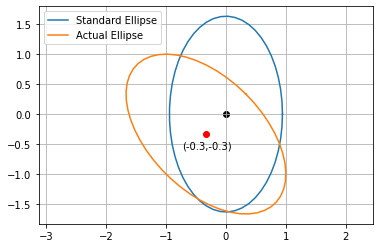
\includegraphics[width=\columnwidth]{solutions/41/18/ellipse.png}
    \caption{Standard Ellipse centered at origin and Actual Ellipse centered at $(-0.3,-0.3)$.}
    \label{eq:solutions/41/18/tangent}
\end{figure}
